\chapter{Distribución $ \chi^2 $}
En estadística, la distribución de Pearson, llamada también ji cuadrada(o) o chi cuadrado(a) ($ \chi^2 $), es una distribución de probabilidad continua con un parámetro  k que representa los grados de libertad de la variable aleatoria

\section{Descripción}
En realidad la distribución ji-cuadrada es la distribución muestral de $s^2$. O sea que si se extraen todas las muestras posibles de una población normal y a cada muestra se le calcula su varianza, se obtendrá la distribución muestral de varianzas. \cite{wiki:4}

\section{PDF}
\begin{center}
	$\frac {(1/2)^{k/2}}{\Gamma (k/2)} x^{k/2-1}e^{-x/2}$
\end{center}

\subsection{Parámetros}
		
\section{CDF}
\begin{center}
	$\frac {\gamma (k/2,x/2)}{\Gamma (k/2)}$
\end{center}

\section{MGF}
\begin{center}
	$(1-2\,t)^{-k/2}$
\end{center}

\section{Media y Varianza}
\subsection{Media}
\begin{center}
	$E(X) = k$
\end{center}

\subsection{Varianza}
\begin{center}
	$var(X) = 2k$
\end{center}

\section{Gráficas}
\begin{center}
	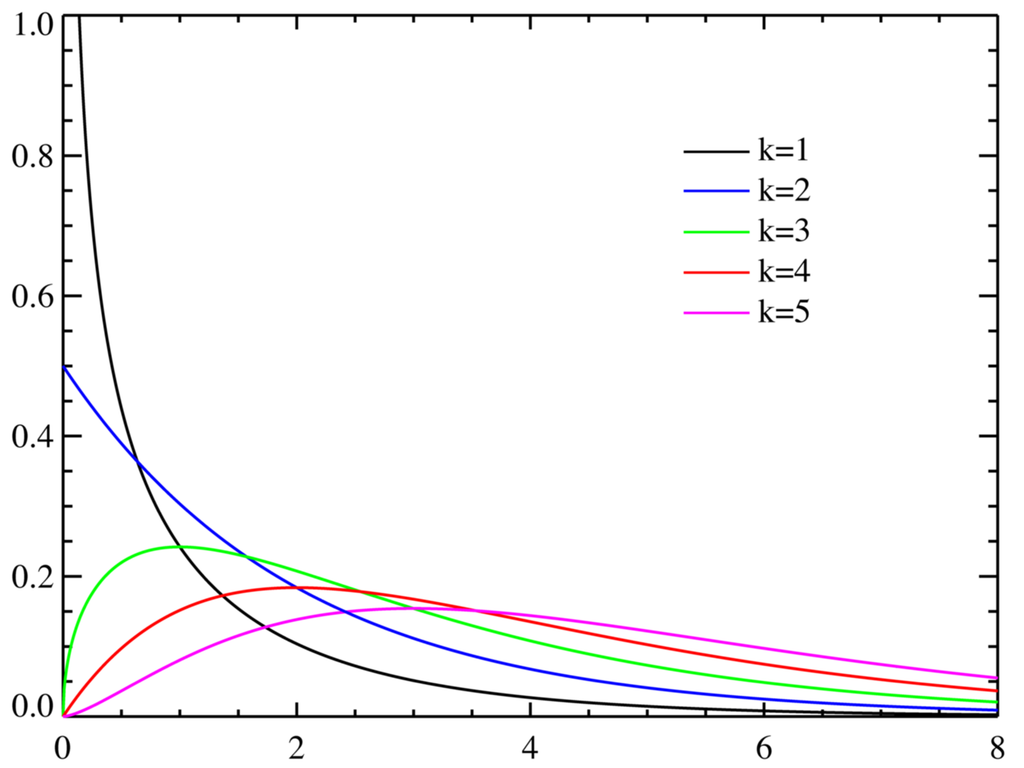
\includegraphics[scale=0.5]{imgs/chi-pdf.png}
	
	\textit{PDF}
\end{center}

\begin{center}
	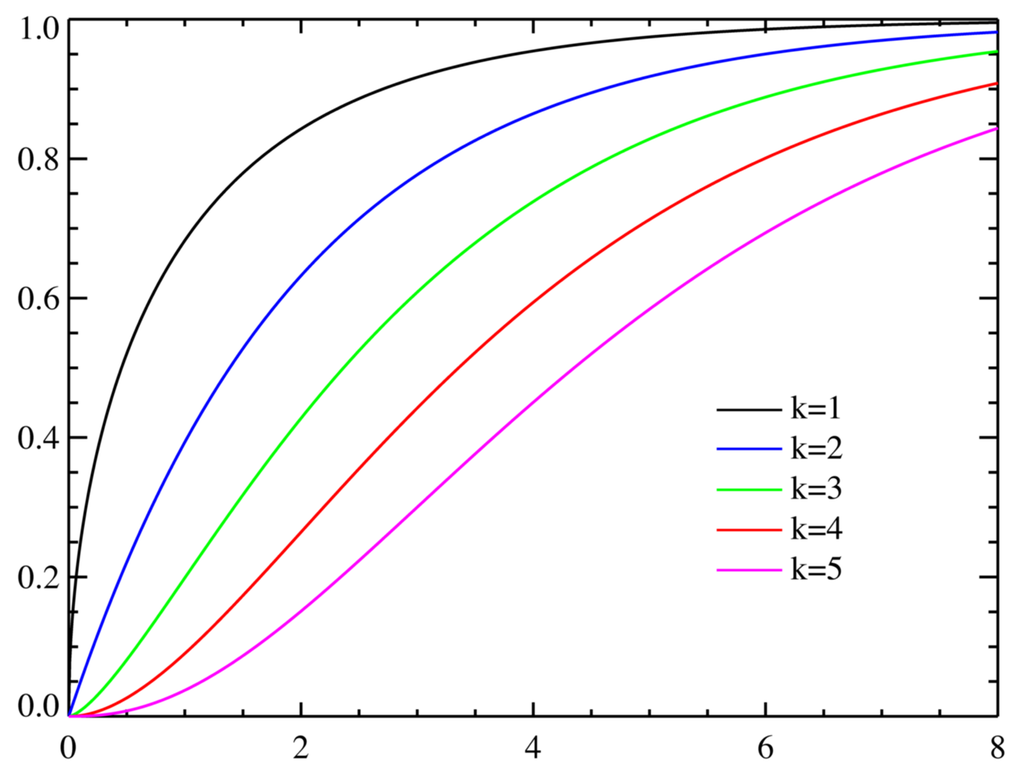
\includegraphics[scale=0.5]{imgs/chi-cdf.png}
	
	\textit{CDF}
	\end{center}

\section{Aplicaciones en la vida real}
Utilizada como prueba de independencia y como prueba de bondad de ajuste y en la estimación de varianzas. Pero también está involucrada en el problema de estimar la media de una población normalmente distribuida y en el problema de estimar la pendiente de una recta de regresión lineal, a través de su papel en la distribución t de Student.